\documentclass[11pt]{report}
\usepackage[utf8]{inputenc}
\usepackage{babel}
\babelprovide[main,import]{spanish}
\usepackage{amsmath,amssymb}
\usepackage{geometry}
\geometry{margin=2.3cm}
\usepackage{setspace}
\onehalfspacing
\usepackage{booktabs}
\usepackage{tikz}
\usepackage{pgfplots}
\pgfplotsset{compat=1.18}
\usepackage{hyperref}
\renewcommand{\thesection}{\arabic{section}}

\title{Mapa de plataformas: figura de m\'erito $\kappa_{1}/\kappa_{2}$ y requisito t\'ermico\\ para los esquemas con qubit de simetr\'ia de inversi\'on rota}
\author{Jhon Sebasti\'an Garc\'ia Barrera}
\date{Septiembre de 2026}

\begin{document}
\maketitle

\section{Criterios}

Se usan tres cantidades, todas calculadas con los par\'ametros publicados por cada trabajo.

\paragraph{Validez perturbativa.} La teor\'ia efectiva exige $\kappa,g_{x},g_{z}\ll\omega$. Se reporta $\kappa/\omega$, $g_{x}/\omega$ y $g_{z}/\omega$.

\paragraph{Figura de m\'erito.} Con $G=2g_{x}g_{z}/\omega$ y $\kappa_{2}=4G^{2}/\kappa$, la p\'erdida de un fon\'on mediada por el qubit es $\Gamma_{1}=g_{x}^{2}\kappa[(\omega^{2}+\kappa^{2}/4)^{-1}+(9\omega^{2}+\kappa^{2}/4)^{-1}]$, y con baño plano y $\kappa\ll\omega$,
\begin{equation}
\frac{\Gamma_{1}}{\kappa_{2}}\simeq\frac{5}{72}\left(\frac{\kappa}{g_{z}}\right)^{2}.
\end{equation}
La tasa total de un fon\'on es $\kappa_{1}=\Gamma_{1}+\gamma$, con $\gamma$ la p\'erdida intr\'inseca del oscilador. El umbral del c\'odigo de repetici\'on de gatos corresponde a $\kappa_{2}/\kappa_{1}=220$ \cite{GuillaudMirrahimi2021}, es decir $\kappa_{1}/\kappa_{2}\leq4.5\times10^{-3}$. Solo por el canal mediado por el qubit, eso exige
\begin{equation}
\boxed{\frac{g_{z}}{\kappa}\geq\sqrt{\frac{5}{72}\cdot220}=3.9},
\end{equation}
y $g_{z}/\kappa\geq8.3$ para $\kappa_{1}/\kappa_{2}=10^{-3}$. Cuando $\kappa_{2}/\kappa\gtrsim0.25$ el confinamiento no lo fija $\kappa_{2}$ sino la tasa de confinamiento f\'isica (Tareas 35, 38 y 47), que satura; se reporta tambi\'en $\kappa_{1}$ dividido entre esa tasa medida. El umbral de Guillaud y Mirrahimi est\'a formulado con $\kappa_{2}$ en el r\'egimen adiab\'atico, as\'i que la comparaci\'on con la tasa de confinamiento es solo orientativa.

\paragraph{Requisito t\'ermico.} Con $n_{q}=[\exp(hf_{q}/k_{B}T)-1]^{-1}$, las Tareas 36 y 37 dan, para el esquema de Naseem en $\Gamma_{2}/\kappa=0.13$, los umbrales de la Tabla~\ref{tab:termico}. Dependen del r\'egimen de acoplamiento (Tarea 44) y deben leerse como orientativos fuera de \'el.

\begin{table}[h]
\centering
\begin{tabular}{ccccc}
\toprule
sesgo $\eta$ & $n_{q}^{*}$ ($|\alpha|^{2}=2$) & $hf_{q}/k_{B}T$ & $n_{q}^{*}$ ($|\alpha|^{2}=3$) & $hf_{q}/k_{B}T$\\
\midrule
100 & $1.5\times10^{-4}$ & 8.8 & $4.2\times10^{-4}$ & 7.8\\
10 & $1.7\times10^{-3}$ & 6.4 & $4.6\times10^{-3}$ & 5.4\\
1 & $2.1\times10^{-2}$ & 3.9 & $9.1\times10^{-2}$ & 2.5\\
\bottomrule
\end{tabular}
\caption{Umbrales t\'ermicos (Tarea 36), expresados en la frecuencia del qubit, $f_{q}=2f_{m}$.}
\label{tab:termico}
\end{table}

\section{Par\'ametros y resultados}

\begin{table}[h]
\centering
\small
\begin{tabular}{lccc}
\toprule
 & Ma et al.~\cite{Ma2019} & Naseem~\cite{Naseem2026} & Liu et al.~\cite{Liu2025}\\
\midrule
plataforma & microondas & mec\'anica & magnones\\
$\omega/2\pi$ & 6 GHz & 100 MHz & 17.7 MHz\\
$g_{x}/2\pi$, $g_{z}/2\pi$ & 212, 212 MHz & 0.6, 6 MHz & 3.54, 3.54 MHz\\
$\kappa/2\pi$ & 30 MHz & 100 kHz & 16 MHz\\
$\gamma/2\pi$ & 0.6 kHz ($Q=10^{7}$) & 15 Hz & 0\\
$f_{q}$ & 12 GHz & 200 MHz & (qubit vestido)\\
\midrule
$\kappa/\omega$ & 0.005 & 0.001 & 0.90\\
$g_{z}/\omega$ & 0.035 & 0.06 & 0.20\\
$g_{z}/\kappa$ & 7.1 & 60 & 0.22\\
$\kappa_{2}/\kappa$ & 1.0 & 2.07 & 0.031\\
$\Gamma_{1}/\kappa_{2}$ & $1.39\times10^{-3}$ & $1.9\times10^{-5}$ & (fuera de validez)\\
$\gamma/\kappa_{2}$ & $2\times10^{-5}$ & $7.2\times10^{-5}$ & 0\\
$\kappa_{1}/\kappa_{2}$ & $1.4\times10^{-3}$ & $9.2\times10^{-5}$ & (fuera de validez)\\
$\kappa_{1}/(\text{confinamiento medido})$ & $1.0\times10^{-2}$ & $8.3\times10^{-4}$ & --\\
$hf_{q}/k_{B}T$ (10 mK) & 58 & 0.96 & --\\
$n_{q}$ (10 mK) & $10^{-25}$ & 0.62 & --\\
\midrule
veredicto & $\kappa_{1}/\kappa_{2}$ bajo umbral, & $\kappa_{1}/\kappa_{2}$ bajo umbral, & fuera del r\'egimen\\
 & confinamiento saturado & falla t\'ermica & perturbativo\\
\bottomrule
\end{tabular}
\caption{Par\'ametros publicados y posici\'on en el mapa. En Ma et al., el disipador $\Gamma[2\sigma_{-}\rho\sigma_{+}-\ldots]$ da $\kappa=2\Gamma$; en Liu et al., $\omega=\nu/2$ con $\nu/2\pi=35.4$ MHz. La tasa de confinamiento medida es 0.14$\kappa$ para Ma (Tarea 43, $|\alpha|^{2}=2$, modelo completo) y 0.23$\kappa$ para Naseem (Tarea 38, criterio de modos estables).}
\label{tab:plataformas}
\end{table}

\paragraph{Ma et al.} Est\'a en el r\'egimen perturbativo. Con $g_{z}/\kappa=7.1$, el cociente adiab\'atico $\kappa_{1}/\kappa_{2}=1.4\times10^{-3}$ queda bajo el umbral, y la f\'ormula coincide con el c\'alculo directo a tres cifras. Pero opera en $\kappa_{2}/\kappa=1$, donde el confinamiento satura en 0.14$\kappa$; con esa tasa el cociente sube a $1.0\times10^{-2}$, por encima del umbral. Reducir $g_{x}$ hasta $\kappa_{2}/\kappa\approx0.1$ conserva $\Gamma_{1}/\kappa_{2}$ (depende solo de $g_{z}/\kappa$) y lleva el confinamiento al r\'egimen donde $\kappa_{2}$ es la tasa correcta. El qubit a 12 GHz no tiene problema t\'ermico.

\paragraph{Naseem.} Con $g_{z}/\kappa=60$, el canal mediado por el qubit es despreciable ($1.9\times10^{-5}$) y domina la p\'erdida intr\'inseca, con $\kappa_{1}/\kappa_{2}=9.2\times10^{-5}$, dos \'ordenes bajo el umbral. Incluso con la tasa de confinamiento saturada el cociente es $8.3\times10^{-4}$. Pero el qubit a 200 MHz tiene $n_{q}=0.62$ a 10 mK, y la Tabla~\ref{tab:termico} exige $hf_{q}/k_{B}T\geq8.8$ para un sesgo de 100: con el qubit a 200 MHz eso requerir\'ia $T\lesssim1.1$ mK, y a 10 mK requiere $f_{q}\gtrsim1.8$ GHz, es decir $\omega_{m}/2\pi\gtrsim0.9$ GHz. Adem\'as, $g_{z}/\omega=0.06$ est\'a en el l\'imite de validez de la transformaci\'on polar\'onica.

\paragraph{Liu et al.} Con $\kappa/\omega=0.9$ y $g_{z}/\omega=0.2$, la jerarqu\'ia $\kappa\ll\omega$ no se cumple y ninguna f\'ormula de este trabajo aplica. La simulaci\'on de su Ec.~(9) (Tareas 46 y 47) no forma el gato que predice su modelo efectivo; se reporta como caso fuera del r\'egimen perturbativo, sin extraer conclusiones sobre su Hamiltoniano completo.

\paragraph{Omitidos.} Hou et al.\ (PRA 110, 013711, 2024) no se incluye porque no tuvimos acceso a sus par\'ametros. El esquema de iones de de Matos Filho y Vogel no pertenece a la clase: su acoplamiento de pares es nativo y la figura de m\'erito no aplica.

\section{Mapa}

\begin{figure}[h]
\centering
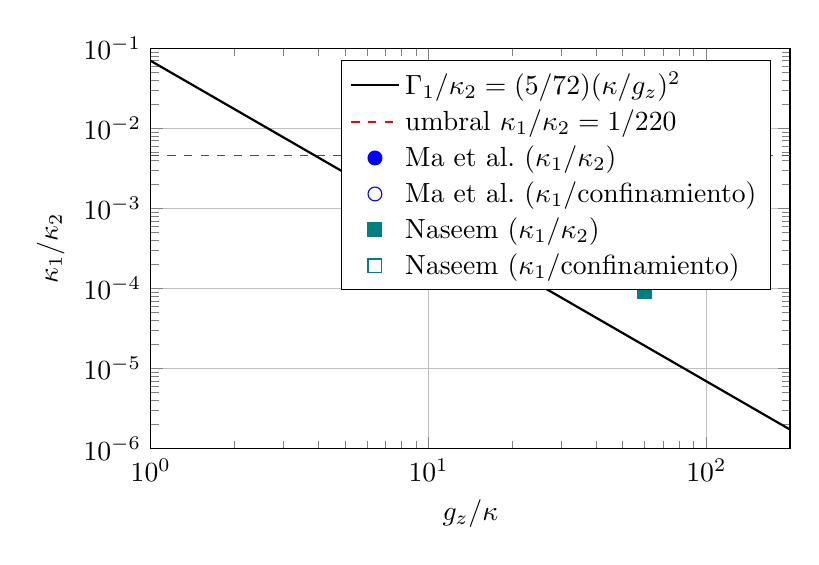
\begin{tikzpicture}
\begin{axis}[width=0.8\textwidth,height=0.55\textwidth,xmode=log,ymode=log,
 xmin=1,xmax=200,ymin=1e-6,ymax=1e-1,xlabel={$g_{z}/\kappa$},ylabel={$\kappa_{1}/\kappa_{2}$},
 legend pos=north east,legend cell align=left,grid=major]
\addplot[black,thick,domain=1:200,samples=100]{5/72/x^2};
\addlegendentry{$\Gamma_{1}/\kappa_{2}=(5/72)(\kappa/g_{z})^{2}$}
\addplot[red,dashed,domain=1:200]{1/220};
\addlegendentry{umbral $\kappa_{1}/\kappa_{2}=1/220$}
\addplot[only marks,mark=*,blue,mark size=2.5pt] coordinates {(7.07,1.409e-3)};
\addlegendentry{Ma et al.\ ($\kappa_{1}/\kappa_{2}$)}
\addplot[only marks,mark=o,blue,mark size=2.5pt] coordinates {(7.07,1.0e-2)};
\addlegendentry{Ma et al.\ ($\kappa_{1}$/confinamiento)}
\addplot[only marks,mark=square*,teal,mark size=2.5pt] coordinates {(60,9.16e-5)};
\addlegendentry{Naseem ($\kappa_{1}/\kappa_{2}$)}
\addplot[only marks,mark=square,teal,mark size=2.5pt] coordinates {(60,8.26e-4)};
\addlegendentry{Naseem ($\kappa_{1}$/confinamiento)}
\end{axis}
\end{tikzpicture}
\caption{Figura de m\'erito frente a $g_{z}/\kappa$. La l\'inea negra es solo el canal mediado por el qubit; los puntos incluyen la p\'erdida intr\'inseca. Liu et al.\ no aparece por estar fuera del r\'egimen perturbativo. El punto de Naseem est\'a bajo el umbral, pero su esquema falla por temperatura, que no se representa en este plano.}
\end{figure}

\section{Conclusiones}

\begin{enumerate}
\item La condici\'on de dise\~no para el canal mediado por el qubit es $g_{z}/\kappa\gtrsim4$ (umbral) u 8 (para $10^{-3}$). Los dos esquemas en r\'egimen perturbativo la cumplen.
\item El confinamiento saturado puede empeorar el cociente efectivo en un orden de magnitud (Ma); la receta es operar con $\kappa_{2}/\kappa\lesssim0.1$ reduciendo $g_{x}$, lo que no cambia $\Gamma_{1}/\kappa_{2}$.
\item La restricci\'on que decide en plataformas de baja frecuencia es la t\'ermica: $hf_{q}/k_{B}T\gtrsim9$ para un sesgo de 100 con $|\alpha|^{2}=2$.
\item Correcci\'on a un valor citado antes en la conversaci\'on: el criterio t\'ermico no es $hf_{q}/k_{B}T\gtrsim5$ sino $\approx8.8$ para sesgo 100 ($\approx5.4$ corresponde a sesgo 10 con $|\alpha|^{2}=3$). El valor 4.8 de la Tarea 37 est\'a expresado en la frecuencia mec\'anica ($hf_{m}/k_{B}T$), no en la del qubit.
\end{enumerate}

\bibliographystyle{unsrt}
\bibliography{refs_mapa}
\end{document}
